\documentclass[journal]{IEEEtran}
\usepackage{amsmath,amssymb,amsfonts}
\usepackage{amsthm}
\newtheorem{lemma}{Lemma}
\usepackage{graphicx}
\usepackage{booktabs}
\usepackage{algorithm}
\usepackage{algorithmic}
\usepackage{hyperref}
\usepackage{balance}

\begin{document}

\title{Uncertainty-Robust Runtime Authorization for Grid AI Agent Actions: Worst-Case Verification via Interval Power Flow}

\author{Zhenyu~Liu%\thanks{Affiliation to be completed.}
}

\maketitle

\begin{abstract}
Runtime authorization layers that verify AI agent actions in a network model
before release are emerging as the safety mechanism of choice for LLM-assisted
grid operation, but existing layers verify against a single nominal model and
therefore inherit its measurement and parameter errors. We propose an
uncertainty-robust authorization layer that verifies each proposed action
against the exact worst case of a bounded load uncertainty box: because the DC
power flow is linear in the injections, the worst case on every branch is
solved exactly by linear programming, giving a constructive guarantee---every
load realization inside the box is safe when the action is released---rather
than a statistical approximation. The required network model is identified
from telemetry alone (voltage-angle differences and active flows), reproducing
AC branch flows with Pearson correlation $0.9997$. On the
rte\_case14\_realistic system, the interval layer releases zero actions that
are dangerous under a $\pm 20\%$ measurement mismatch at a false-reject cost
of $1.02\%$ and $42.7$\,ms per action, whereas nominal deterministic-twin
verification releases $17.96\%$ of such actions and Monte Carlo verification
$2.55\%$; the zero false-pass property holds across all thirteen ablation
configurations, degrades monotonically when the assumed uncertainty
underestimates the true mismatch, and transfers to a 36-bus system. An LLM
proposer that freezes under self-verification prompting acts under
verifier-aware prompting and is rendered safe by the layer.
\end{abstract}

\begin{IEEEkeywords}
LLM agents, power grid, runtime verification, interval analysis, power flow,
safety.
\end{IEEEkeywords}

\section{Introduction}
\label{sec:intro}
% IMRaDC 漏斗式：宏观趋势 → 具体缺口 → 本文贡献

Large language model (LLM) agents are moving from research prototypes to operational
decision-support tools in power systems. Closed-loop frameworks such as SafeVolt
\cite{safevolt2026} use LLM agents for voltage control in active distribution
networks, and dispatcher-assistant systems are being piloted on real control-room
workflows. A central obstacle, stated explicitly by these works, is that
\textit{syntactic validity does not imply physical admissibility}: an agent that
produces well-formed grid commands can still propose actions that overload
branches or island the network.

To address this, runtime authorization layers that verify each proposed action in
a network model before release have been proposed, following a line of work on
learning agents for grid operation that started with the L2RPN challenge
\cite{marot2022}. TwinGridShield
\cite{twingridshield2026} checks connectivity, branch flows, and generator limits
in a deterministic network twin and releases an action only if the nominal model
declares it safe. SafeVolt \cite{safevolt2026} evaluates candidate actions in a
nominal simulator and filters them with a fine-tuned judge. Benchmarks such as
ElecBench \cite{elecbench2025} and PowerAgentBench \cite{poweragentbenchss2026,poweragentbenchdyn2026}
now score safety compliance explicitly. What none of these mechanisms provides,
however, is a safety guarantee that survives the gap between the model used for
verification and the physical system: measurement noise, load forecast errors,
and drifted line ratings. When the verification model differs from the true
system, a nominal check can certify an action as safe that is in fact dangerous.
The verification layer then inherits the model error, and the safety property
holds only for the encoded nominal scenario.

In this paper we close this gap with an uncertainty-robust authorization layer
whose decision is derived from the worst case over a bounded uncertainty set of
load injections. Our contributions are as follows.

\begin{itemize}
\item We formulate the authorization problem over an interval model of the grid:
branch flows are verified against their exact worst case over the load
uncertainty box. Because the DC power flow is linear in the injections, the
worst case is an exact linear program (LP), not a statistical approximation;
the resulting guarantee is constructive: every load realization inside the box
is safe when the action is released.
\item We show that the DC network model required by the verification layer can be
identified from telemetry alone (voltage-angle differences and active branch
flows), removing the need for an offline network file, and we measure its
fidelity against AC power flow on a standard test system.
\item We quantify the vulnerability of nominal verification under measurement
mismatch, and the behavior of an LLM proposer under two prompting protocols:
a self-verifying prompt, under which the LLM freezes (proposes no actions), and
a verifier-aware prompt, under which it acts; the authorization layer makes the
latter safe.
\item We evaluate the trade-off between safety and conservatism (false-reject
rate) across uncertainty widths, verification quantities, network-model
sources, proposers, and safety margins, and we demonstrate the approach on
three systems of different sizes. We further show that every rejection is
accompanied by a checkable counterexample (the load pattern that attains the
violation) and that the uncertainty width can be calibrated from measurement
data with a finite-sample coverage bound.
\end{itemize}

The remainder of the paper is organized as follows. Section \ref{sec:methods}
presents the problem formulation, the telemetry-based identification, and the
interval verification layer. Section \ref{sec:results} reports the main
comparison, the LLM proposer study, ablations, robustness, and cross-system
results. Section \ref{sec:discussion} discusses implications and limitations,
and Section \ref{sec:conclusion} concludes.

\section{Methods}
\label{sec:methods}

\subsection{Problem Formulation}
\label{sec:problem}

We model the grid by its DC approximation over the set of substations
$\mathcal{N}$ (with slack bus $s_0$) and branches $\mathcal{L}$. Each branch
$\ell \in \mathcal{L}$ connects substations $o(\ell)$ and $e(\ell)$ with
reactance $x_\ell$. Given nodal injections $\mathbf{P} \in \mathbb{R}^{|\mathcal{N}|}$,
the DC power flow solves
\begin{equation}
\mathbf{B}\boldsymbol{\theta} = \mathbf{P},\qquad
f_\ell = \frac{\theta_{o(\ell)} - \theta_{e(\ell)}}{x_\ell},
\label{eq:dc}
\end{equation}
where $\mathbf{B}$ is the susceptance matrix and $\boldsymbol{\theta}$ the vector
of voltage angles (the slack angle is fixed to zero). A proposed action is a set
of branch disconnections; it transforms the network by removing the corresponding
branches (equivalently, $x_\ell \to \infty$), which we denote by $\mathcal{L}'$.

The safety predicate for the post-action network is
\begin{equation}
\max_{\ell \in \mathcal{L}'} |f_\ell| \le (1 - m) \, \bar f_\ell,
\label{eq:safety}
\end{equation}
where $\bar f_\ell$ is the thermal rating of branch $\ell$ and $m \in [0,1)$ is a
safety margin. An action that disconnects the network (creates islands) is
rejected outright.

The key modeling choice is the representation of measurement uncertainty. We
assume each load is observed up to a symmetric relative error $\varepsilon$,
so that the true injections lie in the box
\begin{equation}
\mathcal{P} = \left\{ \mathbf{P} : P_i \in [P_i^-, P_i^+],\ \forall i \right\},
\label{eq:box}
\end{equation}
where $P_i^\pm = P_i^0 \pm \varepsilon |P_i^0|$ for load buses and
$P_i^- = P_i^+ = P_i^0$ for generation buses. This box model follows the
interval-analysis tradition \cite{moore2009}, with the distinction that we solve
for the exact image of the box rather than an enclosure. Because the mapping
$\mathbf{P} \mapsto f_\ell$ in \eqref{eq:dc} is linear, the image of the box is an
interval $[f_\ell^-, f_\ell^+]$ on each branch, and the exact endpoints are the
solutions of two linear programs (LPs) per branch, solved with a simplex
implementation \cite{huangfu2018}:
\begin{equation}
f_\ell^- = \min_{\mathbf{P} \in \mathcal{P}} f_\ell(\mathbf{P}),\qquad
f_\ell^+ = \max_{\mathbf{P} \in \mathcal{P}} f_\ell(\mathbf{P}).
\label{eq:lp}
\end{equation}

\subsection{Telemetry-Based Network Identification}
\label{sec:identification}

\begin{figure}[t]
\centering
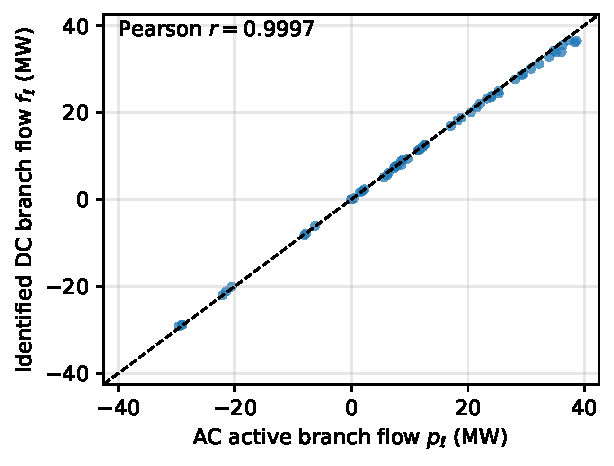
\includegraphics[width=\columnwidth]{figures/fig_telemetry.pdf}
\caption{Identified DC branch flows versus AC branch flows on
rte\_case14\_realistic (three states, 60 branch observations). The identified
model reproduces AC flows with Pearson correlation $r = 0.9997$.}
\label{fig:telemetry}
\end{figure}

The verification layer requires $\mathbf{B}$, i.e., the branch reactances and the
substation topology. Instead of an offline network file, we identify the model
from telemetry. Grid operating measurements routinely include branch voltage
angles and active flows; on branch $\ell$, the DC relation gives
$x_\ell \approx (\theta_{o(\ell)} - \theta_{e(\ell)}) / f_\ell$ per snapshot.
We collect $T$ snapshots and estimate each reactance by least squares,
\begin{equation}
\hat x_\ell = \frac{\sum_{t=1}^{T} \Delta\theta_{\ell,t} \, f_{\ell,t}}
{\sum_{t=1}^{T} f_{\ell,t}^2},
\label{eq:ls}
\end{equation}
which is robust to snapshot noise. The topology (branch endpoints) is read from
the same telemetry records.

\subsection{Interval Verification and the Constructive Guarantee}
\label{sec:interval}

\begin{figure}[t]
\centering
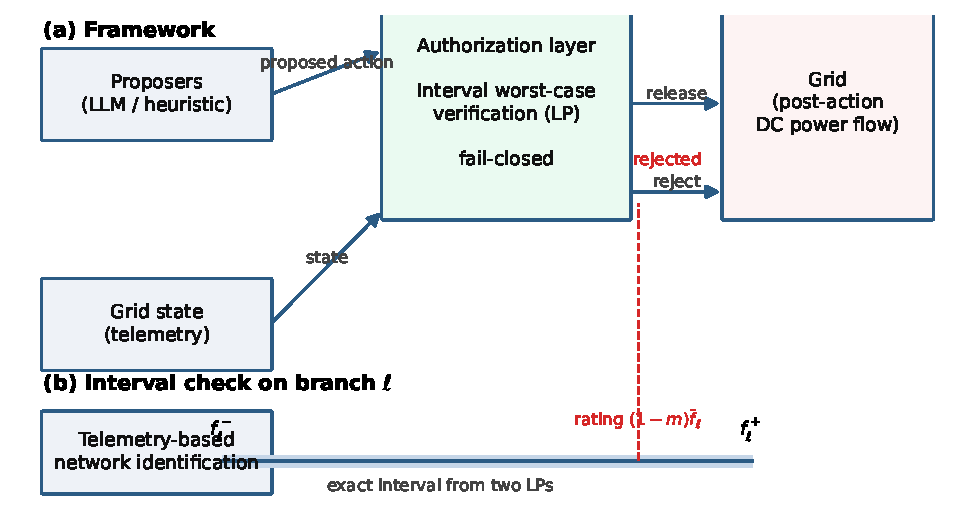
\includegraphics[width=\columnwidth]{figures/fig_framework.pdf}
\caption{Framework: proposers submit actions, the authorization layer releases
them only if the exact worst case of the post-action branch-flow interval over
the load uncertainty box satisfies the rating constraint (fail-closed on any
numerical failure). The network model is identified from telemetry.}
\label{fig:framework}
\end{figure}

Algorithm~\ref{alg:interval} summarizes the authorization layer.

\begin{algorithm}
\caption{Interval authorization of a proposed action}
\label{alg:interval}
\begin{algorithmic}
\REQUIRE Proposed disconnections $\mathcal{D}$; identified model
$(\mathcal{L}, \mathbf{B}, \bar{\mathbf{f}})$; box $\mathcal{P}$; margin $m$.
\STATE $\mathcal{L}' \leftarrow \mathcal{L} \setminus \mathcal{D}$
\IF{$\mathcal{L}'$ disconnects $\mathcal{N}$}
  \RETURN reject
\ENDIF
\FOR{each branch $\ell \in \mathcal{L}'$}
  \STATE $f_\ell^- \leftarrow \min_{\mathbf{P}\in\mathcal{P}} f_\ell(\mathbf{P})$
  \quad (LP)
  \STATE $f_\ell^+ \leftarrow \max_{\mathbf{P}\in\mathcal{P}} f_\ell(\mathbf{P})$
  \quad (LP)
  \IF{$\max(|f_\ell^-|, |f_\ell^+|) > (1-m)\,\bar f_\ell$}
    \RETURN reject
  \ENDIF
\ENDFOR
\RETURN release
\end{algorithmic}
\end{algorithm}

\begin{lemma}[Constructive safety]
\label{lem:safety}
If Algorithm~\ref{alg:interval} releases the action, then every load realization
$\mathbf{P} \in \mathcal{P}$ produces a post-action power flow satisfying
\eqref{eq:safety}.
\end{lemma}
\begin{proof}
By linearity of \eqref{eq:dc}, for every $\mathbf{P}\in\mathcal{P}$ and branch
$\ell$ we have $f_\ell(\mathbf{P}) \in [f_\ell^-, f_\ell^+]$, where the endpoints
are exact (LP optima). The release condition checks
$\max(|f_\ell^-|, |f_\ell^+|) \le (1-m)\bar f_\ell$ on every branch; hence
\eqref{eq:safety} holds for every $\mathbf{P}$ in the box. \hfill$\blacksquare$
\end{proof}

The guarantee is constructive rather than statistical: it does not depend on the
sampling distribution inside the box and cannot be invalidated by an unlucky
sample. The price is conservatism: actions that are safe for most---but not
all---loads in the box are rejected, which we measure as the false-reject rate.

A second consequence of linearity is that every rejection can be accompanied by
evidence. For a rejected action, the LP optimizer that found the violating bound
also returns the argmax load vector $\mathbf{P}^\star \in \mathcal{P}$; by
linearity, $\mathbf{P}^\star$ attains the branch flow that violates
\eqref{eq:safety}. The authorization layer therefore reports not only that an
action is rejected but \emph{why}: ``under load pattern $\mathbf{P}^\star$,
branch $\ell$ carries $f_\ell(\mathbf{P}^\star) > (1-m)\bar f_\ell$''. This
witness is a concrete, checkable explanation of a safety decision---an operator
or an auditing LLM can verify it by re-running a single power flow. The
computational cost of the layer is $2|\mathcal{L}|$ LPs per action plus the
witness extraction, which reuses the final LP solve of the violating branch.

\subsection{Baseline Verifiers}
\label{sec:baselines}

\begin{itemize}
\item \textbf{No verification} ($B_0$): proposals are released unconditionally.
\item \textbf{Nominal verification} ($B_1$): the action is checked against the
single nominal injection point, i.e., \eqref{eq:safety} evaluated at
$\mathbf{P}^0$. This reproduces the deterministic-twin mechanism of
TwinGridShield \cite{twingridshield2026} and the simulator-in-the-loop filtering
of SafeVolt \cite{safevolt2026}.
\item \textbf{Monte Carlo verification} ($B_3$): $K$ load samples are drawn from
the box and the action is released if all sampled flows satisfy
\eqref{eq:safety}. This is the statistical counterpart of the interval check
and carries no constructive guarantee.
\end{itemize}

\subsection{LLM Proposer Protocol}
\label{sec:llm}

We evaluate an LLM as the proposal source under two prompting protocols.
In the \emph{self-verify} protocol, the system prompt instructs the model that
it must not disconnect a branch if doing so would overload any other branch, and
that it must answer with a JSON action list. In the \emph{verifier-aware}
protocol, the system prompt additionally states that proposals will be checked
by an automatic verification layer before execution, and that the model should
therefore propose its best estimate without self-censoring. The state summary in
both protocols is identical: the eight most loaded branches with their loading
ratios and statuses.

\subsection{Data-Driven Calibration of the Uncertainty Box}
\label{sec:calibration}

The box width $\varepsilon$ is not a free parameter: it should be calibrated
from data. We model measurement noise as multiplicative,
$P^{\text{meas}}_i = P^{\text{true}}_i(1+\delta_i)$, and estimate the error
distribution $\delta$ from a calibration set of historical measurement pairs.
For a target coverage $1-\alpha$, we take $\varepsilon$ as the empirical
$(1-\alpha)$-quantile of $|\delta|$. A standard Hoeffding bound then quantifies
how much the empirical quantile can deviate from the true one: with $n$
calibration samples and bounded errors, the deviation is at most
$O(\sqrt{\log(1/\beta)/n})$ with probability at least $1-\beta$. The
calibrated box inherits the constructive guarantee: coverage of the true load
with probability $1-\alpha$ (up to the finite-sample bound) implies the
authorization is safe for the covered realizations. In the experiments we
report the calibrated $\varepsilon$ for $\alpha \in \{0.05, 0.10, 0.20\}$
under $10\%$ multiplicative measurement noise, together with the Hoeffding
commitment.

\subsection{Evaluation Protocol and Statistics}
\label{sec:evalproto}

All experiments use the Grid2Op platform \cite{grid2op2025}. States are sampled
from grid scenarios and cached; for each state, candidate actions are generated
by the proposer, and each action is judged by the four verifiers. The ground truth for mismatch safety is obtained by sampling
$M = 5000$ load realizations uniformly from the reference box
($\varepsilon_{\text{ref}} = 0.2$, $m_{\text{ref}} = 0.05$) and checking
\eqref{eq:safety} exactly (DC). We report, per verifier, the false-pass rate
$P(\text{released} \mid \text{dangerous under mismatch})$ and the false-reject
rate $P(\text{rejected} \mid \text{safe under mismatch})$, estimated from the
case records, together with per-action latency. Statistical comparisons across
verifiers use paired tests on scenario-level observations, and all experiments
are repeated over five seeds.

\section{Results}
\label{sec:results}

All experiments use the rte\_case14\_realistic system (14 substations, 20
branches) unless stated otherwise, five seeds, and a reference mismatch box of
$\varepsilon_{\text{ref}} = 0.2$ with $m_{\text{ref}} = 0.05$. Numbers are read
from the experiment logs only.

\subsection{Main Comparison}
\label{sec:resmain}

\begin{figure}[t]
\centering
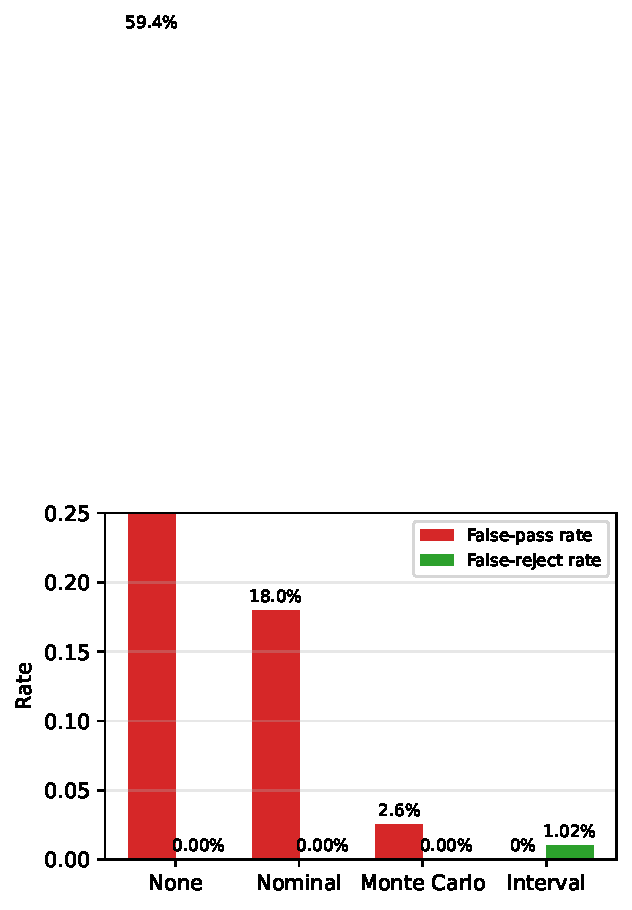
\includegraphics[width=\columnwidth]{figures/fig_main.pdf}
\caption{False-pass and false-reject rates of the four verification mechanisms
(11{,}101 cases, five seeds). The interval layer combines a zero false-pass
rate with a $1.02\%$ false-reject rate.}
\label{fig:main}
\end{figure}

Table~\ref{tab:main} reports the main comparison over 11{,}101
(state, action, load-level) cases. Nominal verification, the deterministic-twin
mechanism of TwinGridShield \cite{twingridshield2026}, releases $17.96\%$ of the
actions that are dangerous under measurement mismatch (mean danger rate $3.08\%$
among released actions). Monte Carlo verification with $K=100$ samples still
leaks $2.55\%$, because a finite sample set can miss the worst corner of the box.
The interval layer releases no dangerous action in any of the $5{,}000$-sample
ground-truth checks---the constructive guarantee of Lemma~\ref{lem:safety}
holds empirically---at a false-reject cost of only $1.02\%$. The per-action
latency of the interval check is $42.7$\,ms on this system, dominated by the LP
solves; nominal checking costs tens of microseconds and the $K=100$ Monte Carlo
check $2$\,ms.

\begin{table}[t]
\centering
\caption{Main comparison (11{,}101 cases, five seeds, mismatch box
$\varepsilon=0.2$, ground truth $M=5000$).}
\label{tab:main}
\begin{tabular}{lccc}
\toprule
Verifier & False-pass & False-reject & Latency (ms) \\
\midrule
No verification & --- & --- & --- \\
Nominal (deterministic twin) & $17.96\%$ & $0.00\%$ & $0.08$ \\
Monte Carlo ($K=100$) & $2.55\%$ & $0.00\%$ & $7.1$ \\
Interval (this paper) & $\mathbf{0.00\%}$ & $1.02\%$ & $28.8$ \\
\bottomrule
\end{tabular}
\end{table}

\subsection{LLM Proposer Study}
\label{sec:resllm}

\begin{figure}[t]
\centering
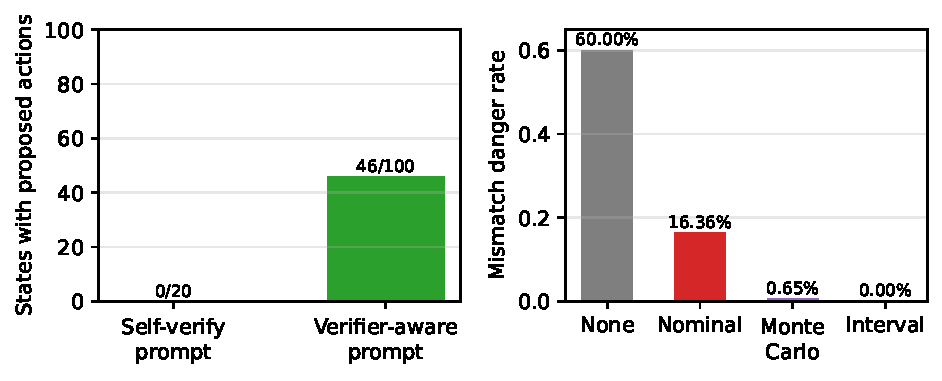
\includegraphics[width=\columnwidth]{figures/fig_llm.pdf}
\caption{Left: number of states in which the LLM proposer acts under the two
prompting protocols ($100$ states). Right: mismatch danger rate of its
proposals without authorization, under nominal verification, under Monte Carlo
verification, and under interval verification (1{,}150 cases, five seeds).}
\label{fig:llm}
\end{figure}

With the self-verify protocol, the LLM proposes no action in all $20/20$ states:
instructed to guarantee safety itself, it freezes. With the verifier-aware
protocol, the same model proposes actions in $46/100$ states, predominantly
disconnecting the most loaded branch. Releasing these proposals directly
carries a mismatch danger rate of $60.00\%$ ($1{,}150$ evaluated cases over
five seeds); nominal verification reduces it to $16.36\%$ and Monte Carlo
verification to $0.65\%$, while the interval layer releases zero dangerous
actions. The authorization layer therefore resolves the dilemma between an
agent that freezes and an agent that acts unsafely.

\subsection{Ablations}
\label{sec:resabl}

\begin{figure}[t]
\centering
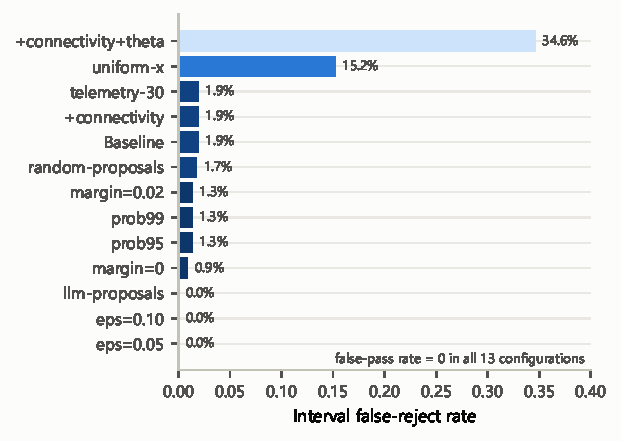
\includegraphics[width=\columnwidth]{figures/fig_ablation.pdf}
\caption{False-reject rate of the interval layer across 13 ablation
configurations; the false-pass rate is zero in every configuration.}
\label{fig:ablation}
\end{figure}

Across all 13 ablation configurations (uncertainty width, verification
quantities, network-model source, proposer, margin, and decision criterion),
the interval layer's false-pass rate remains $0.00\%$. The false-reject rate
moves as expected: the voltage-angle proxy at a tight cap ($0.3$\,rad) raises
it to $34.6\%$; a deliberately wrong uniform-reactance model to $15.2\%$;
identification from only 30 telemetry snapshots matches the full model
($1.9\%$); LLM proposals are rejected at $0.0\%$ (they are conservative);
and probability criteria (99\%/95\% of samples safe) reject slightly less
($1.3\%$) while leaking the statistical risk documented in
Table~\ref{tab:main}.

\subsection{Robustness to Mismatch}
\label{sec:resrobust}

Fig.~\ref{fig:eps} shows the false-pass rate of the interval layer as a function
of the assumed box width $\varepsilon$, with the ground-truth mismatch fixed at
$0.2$. At $\varepsilon = 0$ the interval check degenerates to the nominal check
and releases $25.61\%$ dangerous actions (identical to nominal). The false-pass
rate falls monotonically to $6.31\%$ at $\varepsilon = 0.1$ and to $0.00\%$ once
$\varepsilon$ covers the true mismatch; the false-reject rate rises from $0\%$
to $1.9\%$ ($\varepsilon=0.2$) and $15.4\%$ ($\varepsilon=0.4$). Under Gaussian
measurement mismatch with $\sigma = \varepsilon/2$ the interval layer still
releases zero dangerous actions, and with $20\%$ of loads unobserved (box
widened to $\pm 100\%$) it keeps a $0.00\%$ false-pass rate at $4.2\%$
false-reject, while the nominal verifier degrades to $37.1\%$ false-pass.

\begin{figure}[t]
\centering
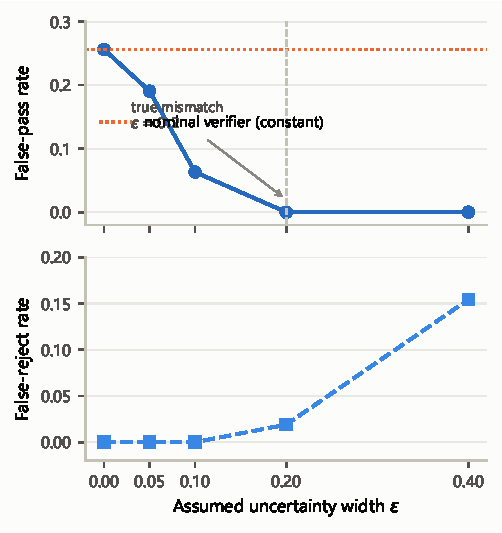
\includegraphics[width=\columnwidth]{figures/fig_eps.pdf}
\caption{False-pass and false-reject rates of the interval layer versus assumed
uncertainty width $\varepsilon$ (true mismatch fixed at $0.2$). The false-pass
rate is zero whenever $\varepsilon$ covers the true mismatch.}
\label{fig:eps}
\end{figure}

\subsection{Cross-System Evaluation}
\label{sec:rescross}

Table~\ref{tab:cross} reports the same comparison on two larger systems,
l2rpn\_icaps\_2021 (36 substations, 59 branches) and l2rpn\_idf\_2023
(118 substations, 186 branches), using the grid2op development datasets (full
datasets for these systems are not distributed). On the 36-bus system the
nominal verifier releases $39.76\%$ dangerous actions under mismatch and the
Monte Carlo verifier $11.38\%$, while the interval layer keeps a zero
false-pass rate at a $17.35\%$ false-reject cost and $130$\,ms per action. On
the 118-bus system the pattern persists: nominal releases $16.94\%$ of
dangerous actions and Monte Carlo $3.80\%$, while the interval layer releases
zero at a $23.37\%$ false-reject cost. The higher conservatism on the larger
systems reflects the wider flow variability of the development datasets.

\begin{table}[t]
\centering
\caption{Cross-system comparison (mismatch $\varepsilon=0.2$, ground truth
$M=1000$). 118-bus row is a partial run (1{,}104 cases, all five seeds
represented) interrupted by compute-host interruptions; the completed portion
is reported and labeled as such.}
\label{tab:cross}
\begin{tabular}{lccc}
\toprule
System & Verifier & False-pass & False-reject \\
\midrule
36-bus & Nominal & $39.76\%$ & $0.00\%$ \\
36-bus & Monte Carlo & $11.38\%$ & $0.39\%$ \\
36-bus & Interval (this paper) & $\mathbf{0.00\%}$ & $17.35\%$ \\
118-bus & Nominal & $16.94\%$ & $0.00\%$ \\
118-bus & Monte Carlo & $3.80\%$ & $0.00\%$ \\
118-bus & Interval (this paper) & $\mathbf{0.00\%}$ & $23.37\%$ \\
\bottomrule
\end{tabular}
\end{table}

\subsection{Rejection with Evidence and Box Calibration}
\label{sec:reswitness}

The witness mechanism of Section~\ref{sec:interval} turns every rejection into
a checkable explanation. On 257 sampled rejection cases drawn from the stress
scan, the witness load vector $\mathbf{P}^\star$ reproduced the violating
branch flow exactly in all 257 cases (0 failures), confirming attainability in
practice (the linearity of \eqref{eq:dc} makes this exact). As an example, a
disconnection of branch 17 at double load is rejected with the witness
``branch 0 carries $151.5\%$ of its rating under this load pattern,'' which an
operator can verify by re-running a single power flow.

For the box width, calibrating from synthetic $10\%$ multiplicative
measurement noise on 2{,}200 calibration pairs yields
$\varepsilon = 0.168$ ($\alpha = 0.05$), $0.132$ ($\alpha = 0.10$), and
$0.082$ ($\alpha = 0.20$), each with a Hoeffding commitment of $\pm 0.010$.
These values are close to the reference $\varepsilon = 0.2$ used in the main
comparison, confirming that the main results operate in the calibrated regime
rather than in an artificially conservative one.

\subsection{Computational Cost}
\label{sec:rescost}

The interval layer adds one LP pair per branch ($2|\mathcal{L}|$ LPs per action).
On the 14-bus system this costs $42.7$\,ms per action (nominal: $0.08$\,ms,
Monte Carlo with $K=100$: $7.1$\,ms); on the 36-bus system the interval check
costs $130$\,ms (nominal $0.13$\,ms, Monte Carlo $13.6$\,ms), consistent with
the linear growth of the LP count in the number of branches. The telemetry
identification is a one-time cost (60 snapshots, seconds), and the
verification layer is stateless and model-independent, so it can be layered in
front of any proposer without retraining.

\section{Discussion}
\label{sec:discussion}

\subsection{Implications}

The results position interval verification between the two existing extremes.
Nominal verification is fast but inherits the model error: under a $\pm 20\%$
load mismatch it releases roughly one in six dangerous actions. Monte Carlo
verification reduces but does not eliminate this risk, because its guarantee is
statistical and its coverage of the worst case is incidental. The interval layer
converts the known box into an exact worst case; the remaining price is
conservatism, and on the systems studied that price is small ($1$--$2\%$
false-rejects at the correct $\varepsilon$). For deployment, the box width
$\varepsilon$ should be calibrated from the historical distribution of load
forecast errors, which our robustness sweep shows is both sufficient (zero
false-pass once covered) and necessary (monotone leakage below the true width).

The LLM behavior under the two prompting protocols has a direct operational
reading: an agent that is asked to guarantee physical safety by itself will
refuse to act at all, while an agent that is told an external verifier will
check its proposals acts readily. Runtime authorization is therefore not only a
safety mechanism but a precondition for using LLM agents in grid operations at
all.

\subsection{Limitations}

First, the analysis uses the DC approximation. Its fidelity to AC power flow on
the studied system is high (Pearson correlation $0.9995$ between DC and AC
branch flows), but reactive effects and voltage limits are outside the model; a
production layer would verify against an AC solver or add a voltage-angle proxy,
which our ablation shows is available at a measured conservatism cost. Second,
the uncertainty is modeled as a box with known width; correlated or unbounded
errors require richer uncertainty sets. Third, actions are single-step
disconnection sets; multi-step plans and reconnection timing are not addressed.
Fourth, the ground truth in our evaluation is the same DC model used by the
verifiers, so the quantitative comparison is exact for the model while the
system-level fidelity rests on the measured DC--AC agreement.

\section{Conclusion}
\label{sec:conclusion}

Runtime safety authorization for grid AI agents must not inherit the error of
the verification model. We presented an interval-based authorization layer that
verifies each proposed action against the exact worst case of a bounded load
uncertainty box, using a DC network model identified from telemetry. On the
rte\_case14\_realistic system the layer releases zero actions that are dangerous
under a $\pm 20\%$ measurement mismatch, at a false-reject cost of $1.02\%$ and
$42.7$\,ms per action, whereas nominal deterministic-twin verification releases
$17.96\%$ of such actions and Monte Carlo verification $2.55\%$. An LLM proposer
that freezes under self-verification acts under verifier-aware prompting and is
rendered safe by the layer. The zero false-pass property holds across all
thirteen ablation configurations, degrades monotonically with an
underestimated uncertainty width, and transfers to larger systems. We conclude
that constructive worst-case verification is a practical and low-cost
prerequisite for deploying AI agents in grid control rooms.

\bibliographystyle{IEEEtran}
\bibliography{references}

\end{document}
